\section{Why the Model Does Not Fit, and How It Is Made To}\label{sec:background}

\paragraph{Why this model.}
On LiveBench~\citep{white2025livebench}, the unquantized model at maximum reasoning effort, as served by DeepSeek,
scores \dv{livebench.deepseek-v4.1-flash-max.All} overall against \dv{livebench.claude-opus-5-5-max-effort.All} for
Claude Opus 5.5 and \dv{livebench.claude-fable-5-1-max-effort.All} for Claude Fable 5.1 at maximum effort. On agentic
coding it is first of the \dv{livebench.n_models} models listed, at
\dv{livebench.deepseek-v4.1-flash-max.Agentic_Coding} against \dv{livebench.agentic.runner_up} for the next
(Figure~\ref{fig:livebench}, Table~\ref{tab:livebench}). The leaderboard data were downloaded on 2026-10-07 and are
stored with hashes in \datafile{data/static/livebench/}~\citep{livebench2026leaderboard}. These are third-party scores
of a different configuration. We serve a \dv{cfg.exl3_bits}-bit pack with thinking disabled, which was not evaluated
on LiveBench, so the scores say why the model is worth serving on modest hardware and are not results of this paper.

\begin{figure}[t]
\centering
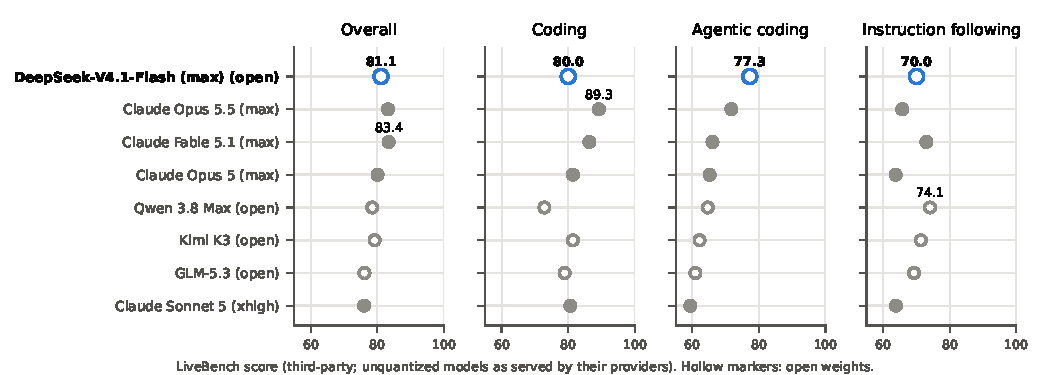
\includegraphics[width=\linewidth]{figures/generated/livebench.pdf}
\caption{Third-party context, not a measurement of this paper: LiveBench scores (question set 2026-06-25, downloaded
2026-10-07) of the unquantized models as served by their providers at the named reasoning effort. DeepSeek-V4.1-Flash
(highlighted) is the maximum-effort, thinking-on configuration. The 3-bit, thinking-off stack studied here was not
evaluated on LiveBench. Hollow markers are open-weight models. Values are labelled for DeepSeek-V4.1-Flash and the best
model of each panel. Source: \datafile{data/static/livebench/}.}
\label{fig:livebench}
\end{figure}

% Generated by hostoffload.analysis.pipeline. Do not edit.
\begin{table}[t]
\centering
\small
\begin{fittable}{tab:livebench}
\begin{tabular}{lrrrr}
\toprule
model & Overall & Coding & Agentic coding & Instruction following \\
\midrule
DeepSeek-V4.1-Flash (max) $^{\circ}$ & 81.1 & 80.0 & 77.3 & 70.0 \\
Claude Opus 5.5 (max) & 83.2 & 89.3 & 71.7 & 65.7 \\
Claude Fable 5.1 (max) & 83.4 & 86.4 & 66.1 & 73.0 \\
Claude Opus 5 (max) & 80.1 & 81.4 & 65.2 & 63.8 \\
Qwen 3.8 Max $^{\circ}$ & 78.5 & 72.9 & 64.6 & 74.1 \\
Kimi K3 $^{\circ}$ & 79.2 & 81.4 & 62.2 & 71.4 \\
GLM-5.3 $^{\circ}$ & 76.1 & 79.0 & 60.9 & 69.3 \\
Claude Sonnet 5 (xhigh) & 76.0 & 80.7 & 59.4 & 63.9 \\
\bottomrule
\end{tabular}
\end{fittable}
\caption{Third-party context: LiveBench scores of the unquantized models as served by their providers at the named reasoning effort (question set 2026-06-25, data downloaded 2026-10-07, \texttt{data/static/livebench/}). $^{\circ}$ open weights. The DeepSeek-V4.1-Flash row is maximum effort with thinking on; the 3-bit stack measured in this paper (thinking off) was not evaluated on LiveBench.}
\label{tab:livebench}
\end{table}


\paragraph{A team of specialists.}
Picture a very large team of specialists, of whom only a few are consulted for any given word. That is a
mixture-of-experts model. Each of DeepSeek-V4.1-Flash's \dv{cfg.num_hidden_layers}
layers~\citep{deepseekai2026v41flash,deepseekai2026v41flashcard} has \dv{cfg.n_routed_experts} routed experts plus
\dv{cfg.n_shared_experts} shared one, and a router sends each token (a piece of a word) to only
\dv{cfg.num_experts_per_tok} of the \dv{cfg.n_routed_experts}. Most specialists are idle at any moment, but all of them
have to be somewhere the GPU can reach, and together they hold most of the model's bytes:
\dv{static.orig.routed_expert_gib}\,GiB of the \dv{static.orig.total_gib}\,GiB checkpoint. The offload rests on that
picture. A specialist who is rarely consulted can wait in a back room, the host's memory, as long as the GPU can still
reach it when the router calls. The rest of this section shows that the back room is necessary on two 96\,GB GPUs and
how the stack uses it.

\paragraph{Making the specialists smaller.}
The first step is compression. EXL3, the format of ExLlamaV3~\citep{turboderp2026exllamav3}, belongs to the
trellis-coded family of QTIP~\citep{tseng2024qtip}. Weights are rotated with Hadamard transforms so that no single
value dominates, then encoded as paths through a trellis with a small codebook, and a GPU kernel decodes them tile by
tile inside the matrix product. The served pack stores the routed experts at \dv{cfg.exl3_bits} bits per
weight~\citep{coolbho3k2026dsv41exl3} and keeps the other weights in DeepSeek's FP8. One routed expert shrinks from
\dv{static.orig.expert_mib}\,MiB in the original checkpoint to \dv{static.expert_mib}\,MiB, and all routed experts
together from \dv{static.orig.routed_expert_gib} to \dv{static.pack.routed_expert_gib}\,GiB.

\paragraph{Compression is not enough.}\label{sec:system}
We accounted every tensor of both checkpoints by class, from their safetensors headers fetched with HTTP range
requests (\dv{static.pack.n_tensors} tensors and \dv{static.pack.total_gib}\,GiB for the pack, with no weights
downloaded), and from placement rules that mirror the documented configuration
(\datafile{src/hostoffload/weights/split.py}, Table~\ref{tab:static-placement}). Even with the large tables and the
embedding in host memory, the pack's GPU-resident weights come to \dv{static.noplan.vram_gib}\,GiB, or
\dv{static.noplan.vram_per_gpu_gib}\,GiB per GPU, against the \dv{expl.gpu_total_gib}\,GiB the driver reports per
card before any KV cache, CUDA graph or activation. That is \dv{expl.noplan_over_per_gpu_gib}\,GiB too much per card.
The original checkpoint is far out of reach, with \dv{static.orig.vram_min_gib}\,GiB outside its Engram tables and
embedding.

% Generated by hostoffload.analysis.pipeline. Do not edit.
\begin{table}[t]
\centering
\small
\begin{fittable}{tab:static-placement}
\begin{tabular}{lrrrrr}
\toprule
tensor class & original & EXL3 pack & VRAM & host & other \\
\midrule
routed experts (40 layers) & 268.95 & 190.48 & 133.34 & 57.14 &  \\
Engram tables & 188.83 & 103.00 & 0.00 & 103.00 &  \\
attention and indexer & 4.80 & 4.80 & 4.80 & 0.00 &  \\
drafter experts & 6.72 & 4.76 & 2.58 & 2.18 &  \\
shared experts & 1.42 & 1.42 & 1.42 & 0.00 &  \\
token embedding & 1.23 & 1.23 & 0.00 & 1.23 &  \\
lm head & 1.23 & 1.23 & 1.23 & 0.00 &  \\
vision tower & 0.90 & 0.90 & 0.00 & 0.00 & not loaded \\
Engram projections & 0.29 & 0.59 & 0.59 & 0.00 &  \\
drafter dense & 0.56 & 0.56 & 0.56 & 0.00 &  \\
routers & 0.15 & 0.15 & 0.15 & 0.00 &  \\
norms, hyper-connections & 0.15 & 0.15 & 0.15 & 0.00 &  \\
\textbf{total} & 475.24 & 309.28 & 144.81 & 163.56 & 0.90 \\
\bottomrule
\end{tabular}
\end{fittable}
\par\smallskip\parbox{0.95\linewidth}{\footnotesize\raggedright Sources: \texttt{data/static/weights/deepseek-ai-2cba9e42/placement.json}, \texttt{data/static/weights/diffbot-a1cf1bd2/placement.json}.}
\caption{Checkpoint bytes by tensor class (GiB, from safetensors headers) for DeepSeek's original checkpoint and the served EXL3 pack, and where the pack's bytes go under the \texttt{gen30} host-expert plan with the documented placement rules (text-only serving). File bytes, not runtime allocations. Static measurement.}
\label{tab:static-placement}
\end{table}


\paragraph{The back room.}
Diffbot's plans close the gap by moving the least-used experts to pinned host memory. All the plans published with the
recipe put \dv{static.gen30.host_target_experts} of the \dv{static.target_experts} target experts on the host
(\dv{static.gen30.host_target_share_pct}\%, between \dv{static.gen30.host_per_layer_min} and
\dv{static.gen30.host_per_layer_max} per layer, Figure~\ref{fig:hostperlayer}). They differ in which experts, chosen
from the routing counts of different traffic. Two other large objects live in the back room in every configuration:
the Engram tables~\citep{cheng2026engram}, two lookup tables indexed by hashed word sequences that give the model
memory by lookup rather than by computation (compressed to int4, from \dv{static.orig.engram_table_gib} to
\dv{static.pack.engram_table_gib}\,GiB), and the token embedding. With the \texttt{gen30} plan the pack's GPU share
drops to \dv{static.gen30.vram_per_gpu_gib}\,GiB per GPU, and \dv{static.gen30.host_gib}\,GiB of file bytes sit on the
host, \dv{static.gen30.host_expert_gib}\,GiB of them experts. Figure~\ref{fig:memarch} shows where everything lives.

The back room is reached without copies. CUDA can register host memory as pinned and map it into the GPU's address
space (unified virtual addressing, or UVA), so that a kernel dereferencing such a pointer reads the data over PCIe, the bus between each GPU and the
computer's main memory, at the moment of use, with no explicit transfer and no cache on the GPU
side~\citep{nvidia2026cudaguide}. This is called zero-copy access. Upstream vLLM already serves the Engram tables this way, and Diffbot's patch does
the same for the cold experts. At each expert layer the patched plugin launches the GPU-resident experts on the main
CUDA stream and the host experts on a second stream limited to a few of the GPU's compute units (SMs), so that the
slow reads over PCIe overlap with the fast work in GPU memory. Because these reads are not copies, a profiler does not
show them as transfers. They appear in the PCIe throughput counters, which our samplers record.

\begin{figure}[t]
\centering
\resizebox{\linewidth}{!}{% Memory architecture of the measured stack. Every number is a \dv value from data/ (static file bytes or the
% exploratory server log). Only the layout is hand-written.
\begin{tikzpicture}[
  font=\footnotesize, >=Stealth,
  box/.style={draw=black!60, rounded corners=1.5pt, align=center, inner sep=3pt, line width=0.4pt},
  vram/.style={box, fill=blue!8},
  host/.style={box, fill=orange!14, text width=4.3cm},
  link/.style={->, line width=0.7pt, draw=black!70}]
  \foreach \g/\x in {0/0, 1/8} {
    \draw[draw=black!60, rounded corners=2pt, fill=black!2] (\x, 0) rectangle (\x+7, 4.6);
    \node[anchor=north west] at (\x+0.1, 4.55) {\textbf{GPU\g}: \dv{expl.gpu_total_gib} GiB, tensor-parallel rank \g};
    \node[vram, text width=6.4cm] (hot\g) at (\x+3.5, 3.45) {hot routed experts (the VRAM part of the plan)\\
      dense layers: attention, indexer, shared experts, routers, lm head};
    \node[vram, text width=2.9cm] (kv\g) at (\x+1.85, 2.15) {fp8 KV cache shard\\ \scriptsize(pool: \dv{expl.kv_tokens} tokens)};
    \node[vram, text width=2.9cm] (cg\g) at (\x+5.15, 2.15) {CUDA graphs\\ \dv{expl.cuda_graph_gib} GiB};
    \node[box, fill=black!6, text width=6.4cm] (sm\g) at (\x+3.5, 0.75) {SMs: main stream runs VRAM experts;\\
      side stream runs host experts on a bounded SM budget};
  }
  \draw[draw=black!60, rounded corners=2pt, fill=black!2] (0, -4.6) rectangle (15, -1.7);
  \node[anchor=south west] at (0.1, -4.55) {\textbf{Host memory}: pinned, registered, mapped into the GPU address
    space (UVA); \dv{expl.cgroup_max_gib} GiB cgroup limit};
  \node[host] (cold) at (2.6, -2.75) {cold routed and drafter experts\\ \dv{static.gen30.host_experts} experts,
    \dv{static.gen30.host_expert_gib} GiB (file)};
  \node[host] (engram) at (7.5, -2.75) {Engram tables, int4\\ \dv{cfg.engram_tables} tables,
    \dv{expl.engram_pinned_gib} GiB, rows sharded by rank};
  \node[host] (emb) at (12.4, -2.75) {token embedding\\ \dv{static.pack.embedding_gib} GiB (file)};
  \draw[link] (cold.north) -- node[pos=0.7, left, align=right, font=\scriptsize] {zero-copy reads\\ over PCIe} (sm0.south);
  \draw[link] (cold.north) -- (sm1.south west);
  \draw[link] (engram.north) -- node[pos=0.7, right, font=\scriptsize, align=left] {row gathers\\ over PCIe} (sm1.south);
  \draw[link] (engram.north) -- (sm0.south east);
  \draw[link, dashed] (emb.north) -- node[pos=0.7, right, font=\scriptsize] {lookups} (sm1.south east);
\end{tikzpicture}
}
\caption{Memory architecture of the measured stack (two GPUs, tensor parallel). Blue: GPU memory (VRAM). Orange:
pinned host memory that GPU kernels read over PCIe by zero-copy access (UVA). Sizes are checkpoint bytes from the safetensors headers
(\datafile{data/static/weights/diffbot-a1cf1bd2/placement.json}) or values the server logged at load in the exploratory
run (KV tokens, CUDA graph memory, Engram tables), all printed from data files.}
\label{fig:memarch}
\end{figure}

\begin{figure}[t]
\centering
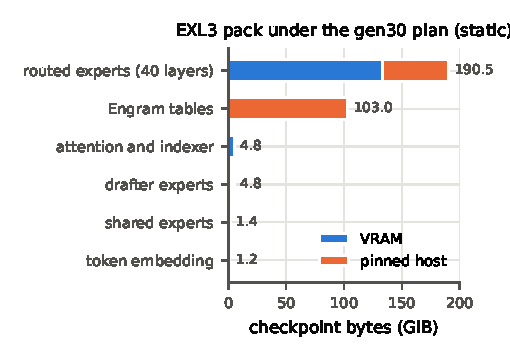
\includegraphics[width=0.49\linewidth]{figures/generated/static_placement.pdf}\hfill
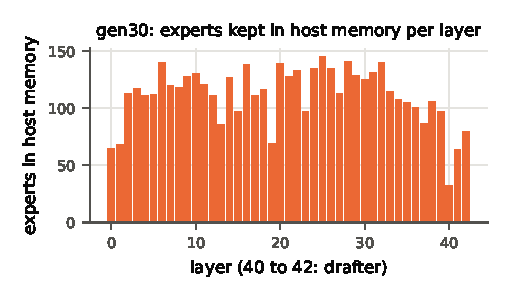
\includegraphics[width=0.49\linewidth]{figures/generated/static_host_per_layer.pdf}
\caption{Static measurement. Left: checkpoint bytes per tensor class in GPU memory and in pinned host memory under the
\texttt{gen30} plan. Right: experts the plan keeps in host memory, per layer (layers 40 to 42 are the drafter).
Source: \datafile{data/static/weights/diffbot-a1cf1bd2/placement.json}.}
\label{fig:hostperlayer}
\end{figure}

\paragraph{Checking the accounting against the server.}
Placement rules are a model, so we checked them where the server reports what it did. The Engram bytes the server
pinned in the exploratory run (\dv{expl.engram_pinned_gib}\,GiB, in four shards of
\dv{expl.engram_per_table_rank_gib}\,GiB) equal the file bytes. The per-layer counts of host experts it logged equal
those of one published plan on every layer, which identifies the plan each exploratory run used
(Section~\ref{sec:results-exploratory}). File bytes are not runtime bytes, though. vLLM reported
\dv{expl.model_loading_gib}\,GiB of weights per GPU, \dv{expl.runtime_minus_file_gib}\,GiB more than the plan's file
bytes in GPU memory, presumably from repacked and duplicated layouts that we did not attribute allocation by
allocation. The exploratory boot also left \dv{expl.headroom_mib}\,MiB of GPU memory unused per card at its peak.
Spending all of it on experts would bring \dv{expl.min_share.movable_experts} of them back, so with this KV budget and
these graph sizes at least \dv{expl.min_share.pct}\% of the target experts must stay on the host. That is an estimate
from one boot, and no run searched for the smallest share that boots.

\paragraph{The boots.}
Experiment E2 tested the accounting on the GPUs (Table~\ref{tab:ctl-E2}). The EXL3 plugin with every expert in GPU
memory and the offload build with an empty plan both stopped while loading, with the server's own out-of-memory
errors. The same offload build with the \texttt{gen30} plan booted and served all the measurements of the next
sections. The byte accounting (E0) and the boots (E2) are specified in Section~\ref{sec:method}, and the pods they ran
on in Section~\ref{sec:setup}.

% Generated by hostoffload.analysis.pipeline. Do not edit.
\begin{table}[t]
\centering
\small
\begin{fittable}{tab:ctl-E2}
\begin{tabular}{lllp{6cm}}
\toprule
configuration & status & failure & first error line \\
\midrule
exl3-min-allvram & boot\_failed & gpu\_oom & \texttt{(Worker\_TP1 pid=11812) ERROR 10-06 20:04:41 [multiproc\_executor.py:948] torch.OutOfMemoryE} \\
exl3-offload-noplan & boot\_failed & gpu\_oom & \texttt{(Worker\_TP1 pid=15785) ERROR 10-06 20:08:11 [multiproc\_executor.py:948] torch.OutOfMemoryE} \\
\bottomrule
\end{tabular}
\end{fittable}
\caption{Controlled: feasibility boots on 2x RTX PRO 6000 (E2). Status and the first matching error line of the server log (\texttt{hostoffload.analysis.failures}).}
\label{tab:ctl-E2}
\end{table}

